\documentclass{article}
\usepackage{graphicx}
\graphicspath{ {./images/} }
\usepackage{parskip}
\usepackage{listings}
\usepackage{color}
\usepackage[utf8]{inputenc}

\renewcommand{\figurename}{Abb.}
\renewcommand{\lstlistingname}{Quelltext}
\renewcommand{\contentsname}{Inhaltsangabe}

\lstset{ 
	language=C++,
	basicstyle=\small\sffamily,
	numbers=left,
 	numberstyle=\tiny,
	frame=tb,
	tabsize=4,
	columns=fixed,
	showstringspaces=false,
	showtabs=false,
	keepspaces,
	commentstyle=\color{green},
	keywordstyle=\color{blue}
}

\begin{document}

\begin{titlepage}
\centering
NVS- Projekt 2020/21, 5AHIF

\vskip2cm
{
	\bfseries\Large
 	\huge\underline{C++ Networking Sliding Window}\\
	Maurice Putz\\
}
\vskip1cm

\includegraphics[width=10cm]{connectsim.png}
\vskip3cm
 11. April 2021\\
\end{titlepage}

\pagenumbering{gobble}
\newpage
\tableofcontents
\newpage
\pagenumbering{arabic}

\section{Beschreibung}
Das Progamm ConnectSim dient dazu, eine Übertragung von Daten mittels einem Sliding Window Algorithmus darzustellen.
Weiters bietet das Programm noch die Funktionen, drei Fehlerarten im Networking darzustellen. Diese wären Paketverlust,
Paketverfäschung (Datenmanulupation) und eine falsche Paketreihenfolge. Vom Sender aus werden zufällige ASCII-Zeichen, deren
Menge optional angeben werden kann, in derer dezimalen Darstellung, mittels einer Verbindung zu einem Server übertragen. Diese
Verbindung ist vordefiniert. Der Server wird vor der Ausführung des Programms manuell vom User gestartet, dieser wartet dann auf einkommende
Verbindungsanfragen und startet den Alogrithmus bei erfolgreicher Verbindung. \newline
Die größe des Sliding Window Fensters veträgt Standardgemäß 1, ist aber per Kommandozeile vom User aus konfigurierbar.
Die Daten weden Client zum Server übertragen. Zuerst wird die Anzahl, aller zu übertrageneder Datenframes, dann die größe des Sliding Window Fensters
dem Server mitgeteilt. Danach beginnt die eigentliche Übertragung der Daten. Der Server nimmt ein Datenframe aus, addiert den Wert zu einer Checksumme 
welche pro Fenster berechnet wird und sendet die Daten, als AKN zurück. Wurden so viele Daten aufgenommen, wie die Sliding Window größe vorher übermittelt worden
ist, sendet der Server einen AKN an den Client mit der gesamten Checksumme des Fensters und alles beginnt wieder von vorne, bis alle Daten auf diese Art übertragen worden
sind.\newline
Am Ende überträgt der Server nochmals die maximale Summer der Übertragenen Daten pro Fenster zum Client. Diese Summe hat sich der Client selbst vor dem Abschicken der
Daten gebildet. Diese wird nun verglichen ob sie dieselbe ist. 
\newline\newline
Das Programm gibt diesen Vorgang in einer Logdatei für den Server, und einer Logdatei für den Client aus. Der Name und Pfad der Logdatei für den Client ist frei konfigurierbar.
Es gibt noch einige weitere Funktionen, wie auch die Simulation von Netzwerkfehlern. Diese werden im Abschnitt "Bedienanleitung", genauer beschrieben.


\subsection{Sliding-Window Algorithmus Zusammenfassung}
Das Sliding Window Protokoll wird für die Übetragung von Informationen benutzt. Eine Beschreibung ist dazu im RFC 1180 zu TCP/IP unter Absatz 7 TCP (Transmission Control Protocol).
Im Grunde genommen bewirkt dieser Algorithmus, dass ein Client mehrer Datenframes auf einmal versenden kann, ohne das er auf ein AKN des Servers warten muss. Eine genauere Grafische Darstellung,
wie das Fenster über die Daten "schiebt" zeigen folgende Abb. 1 bis inklusive Abb. 3.

\begin{center}
\begin{figure}[h]
    \centering
    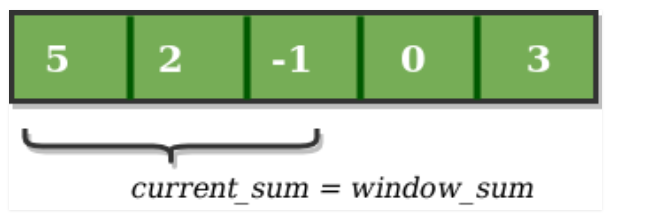
\includegraphics[width=\textwidth]{slidingwindow1.png}
    \caption{Ausgangsposiiton mit Fenstergröße 3}
\end{figure}
\end{center}
\break

Das Fenster hat die immer die Größe 3, die Summe aller Daten im dargestellten Fenster beträgt 6. Diese Zwischensumme wird in einer Variable max\_sum zwischengespeichert, nämlich
setzen wir diese gleich dem Wert in current\_sum, dies ist die Summe welche 6 beträgt. Weiter geht es mit dem Schritt in Abbildung 2.

\begin{center}
\begin{figure}[h]
    \centering
    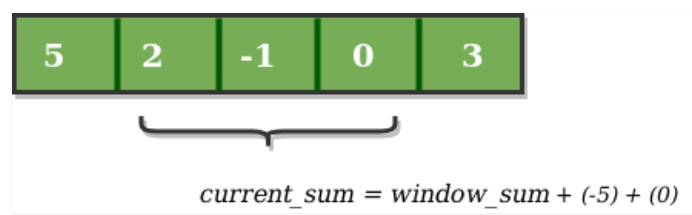
\includegraphics[width=\textwidth]{slidingwindow2.png}
    \caption{Sliding Window um einen Index weitergewandert}
\end{figure}
\end{center}

Nun wischt das Fenster um einen Index weiter nach rechts, in Abb. 2 zu sehen. Der Wert aller Datenframes in dem Bereich des Fensters beträgt nun insgesamt 1. Dies ist kleiner als der Wert in max\_sum. Daher wird der Wert nicht geupdated und das Fenster wischt nochmals weiter, in Abb. 3 zu sehen.

\begin{center}
\begin{figure}[h]
    \centering
    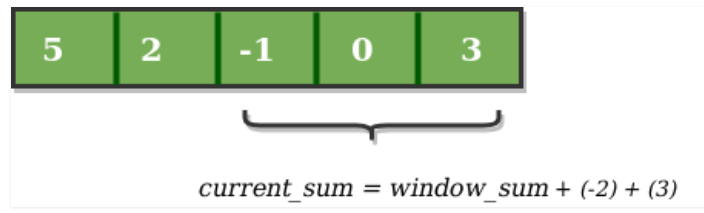
\includegraphics[width=\textwidth]{slidingwindow3.png}
    \caption{Sliding Window um einen Index weitergewandert}
\end{figure}
\end{center}
\break

Nachdem das Fenster wieder um einen Index weitergewandert ist, rechnen wir wieder die summe des Fensters zusammen, in Abb. 3 beträgt die Fenstersumme 2. Nun wird die Summe wieder mit dem Wert in
der Variable max\_sum verglichen. Da der Wert wieder kleiner ist, als der in max\_sum gespeicherte, bleibt max\_sum wie sie ist und unsere maximale Fenstergröße von unserem gesamten Array, ist 6.

\section{Bedienanleitung}
\begin{center}
\begin{figure}[h]
    \centering
    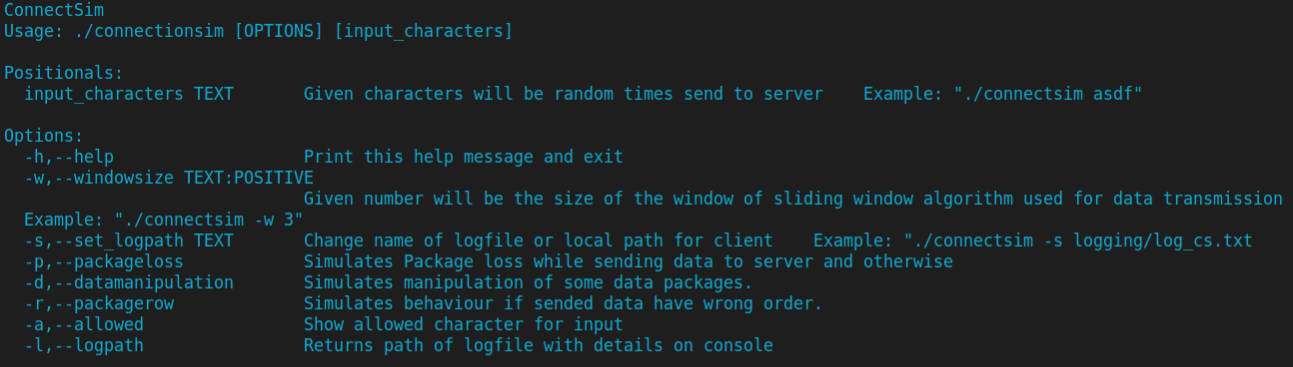
\includegraphics[width=\textwidth]{connectsim-h.png}
    \caption{Übersicht über die Komandozeilenparameter. Befehl: connectsim -h}
\end{figure}
\end{center}

Option \textbf{-h,--help}:\\
Zeigt die Hilfe für das Programm an, liefert das Menü wie in Abb. 4 zurück.
\begin{itemize}
	\item \underline{Eingabe:} ./connectsim -h
	\item \underline{Ausgabe:} [Siehe Abb. 4]\\
\end{itemize}

\break

\subsection{Befehle}
Der Server muss unabhängig vom Programm \textbf{zuerst} gestartet werden und manuell vom User. Dies macht man mittels dem Befehl \underline{./server} in dem Verzeichnis, wo die Datei zum starten
liegt. Eine Abfolge und das Ergebnis sieht man in Abb. 5.

\begin{center}
\begin{figure}[h]
    \centering
    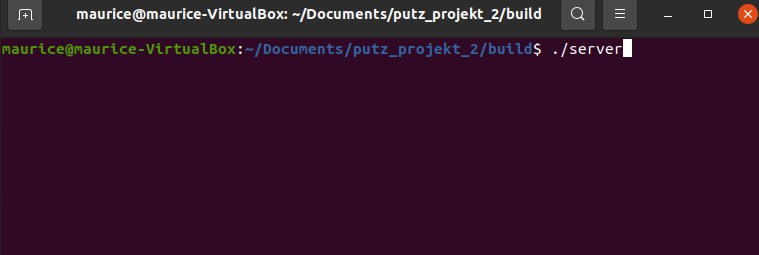
\includegraphics[width=\textwidth]{connectsimserver.png}
    \caption{Startbefehl des Servers}
\end{figure}
\end{center}

Durch den normalen Aufruf des Programms mit \underline{./connectsim}, wird ConnectSim ohne speziellen Funktionen gestartet. Die Standardgröße eines Sliding Window Fensters beträgt eins, welche bei oben gezeigtem Aufruf benutzt wird, die Standardgröße von eins hat auch einen bestimmten Grund, welcher später noch genauer erläutert wird. Das Programm generiert nun zufällig oft zufällig viele (zwischen 1 und 127) ASCII-Charactere und beginnnt die Übertragung. Der Server verarbeitet diese und antwortet. Genauer in den Abb.6-7 zu sehen. Ebenfalls werden ensprechende Ausgaben auf der Konsole der Servers getätigt und in den Logfiles des Servers und des Clients geschrieben.

\begin{center}
\begin{figure}[h]
    \centering
    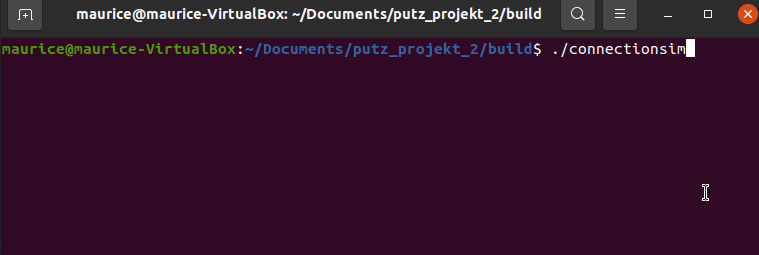
\includegraphics[width=\textwidth]{connectsimclient.png}
    \caption{Startbefehl des Programms}
\end{figure}
\end{center}

\break

\begin{center}
\begin{figure}[h]
    \centering
    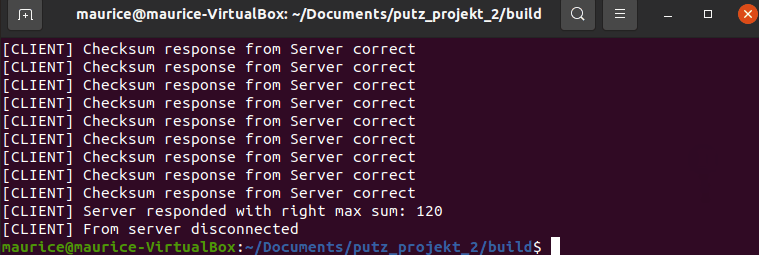
\includegraphics[width=\textwidth]{connectsimcliente.png}
    \caption{Ausgabe von ./connectsim}
\end{figure}
\end{center}

Wenn man beim Aufruf des Programms, wie zum Beispiel  \underline{./connectsim asdf} eingibt, werden die einzelnen Zeichen hinter dem Programmnamen überprüft, ob sie in ASCII enthalten sind und im positiven Fall, wird das Programm genau wie bei einem einfachen Aufruf gestartet. Nur diesmal werden bloß die ASCII-Zeichen, welche hinter dem Programmnamen stehen zufällig oft (zwischen 1 und 127 mal) übertragen.
\newline

\begin{itemize}
	\item \underline{Eingabe:} ./connectsim asdf
	\item \underline{Ausgabe:} Wie bei Abb. 7\newline 
\end{itemize}

Option \textbf{-w,--windowsize TEXT:POSITIVE}:\newline
Startet das Programm und ersetzt die default-Sliding Window Größe auf den angegebenen Wert. Das Programm beendet sich, falls diese Zahl Größer ist, als die Anzahl der zu Übertragenden Elemente. Falls dies der Fall ist, wird eine Nachricht ausgegeben, wie der User in dem Fall verfahren sollte. Zum Beispiel falls der User eine Größe von 8 für das Fenster eingibt, aber durch das Zufallsbedingte auswählen der ASCII Charakter Anzahl nur 5 Charaktere erstellt werden, muss dieser Fall angefangen werden, da die Startbedienungen für den Algorithmus nicht korrekt sind.\\
Erwartet eine positive ganze Zahl als Eingabe.
Beispiel: 
\begin{itemize}
	\item \underline{Eingabe:} ./connectsim -w 3
	\item \underline{Ausgabe:} [Programm startet und Vorgang wird auf der Konsole und in den Logdateien festgehalten]
\end{itemize}

\break

Flag \textbf{-s,--set\_logpath TEXT}:\newline
Setzt den aktuellen Pfad für die Logdatei des Clients, zu dem Angegebenen. Der Pfad wird in der Datei \textbf{settings.json}, abgespeichert.
Erwartet einen einen gültigen Pfad/String als Eingabe.
Beispiel: 
\begin{itemize}
	\item \underline{Eingabe:} ./connectsim -s /new\_folder/client\_log.txt
	\item \underline{Ausgabe:} 
Path of Logging file successfully changed!\\
\end{itemize}

Flag \textbf{-p,--packageloss}:\newline
Simuliert einen Packetverlust. Beim senden vom Client zum Server
Beispiel: 
\begin{itemize}
	\item \underline{Eingabe:} ./connectsim -p
	\item \underline{Ausgabe:} [SERVER] Received package count does not\\ match with received count of data packages to process.
	\\ Please look into log files.\\
\end{itemize}

Flag \textbf{-d,--datamanipulation}:\newline
Simuliert einen Packetverlust. Beim senden von Daten vom Client zum Server.
Beispiel: 
\begin{itemize}
	\item \underline{Eingabe:} ./connectsim -d
	\item \underline{Ausgabe:} [SERVER] Received package count does not\\ match with received count of data packages to process.
	\\ Please look into log files.\\
\end{itemize}

Flag \textbf{-r,--packagerow}:\newline
Simuliert, dass die Reihenfolge der geschickten Packages, falsch ankommt.
Beispiel: 
\begin{itemize}
	\item \underline{Eingabe:} ./connectsim -r
	\item \underline{Ausgabe:} [CLIENT] Server responded with right max sum: [MAX\_SUM of ASCII Characters]\\ oder
	es wird ein "std::system\_error" geworfen und der Server schließt den Socket, so können auf dem Socket keine Daten mehr
	gesendet oder empfangen werden.
\end{itemize}

\break

Flag \textbf{-a,--allowed}:\\
Damit kann man alle erlaubten ASCII Zeichen für das Programm sich anzeigen lassen. Einige ASCII Zeichen wie zum Beispiel 1 - SOH (start of heading), in C++ nicht über die Kommandozeile gewünscht verarbeitet werden kann. Alle Zahlen und Buchstaben und die meisten welche in ASCII enthalten sind, werden unterstützt.

\begin{itemize}
	\item \underline{Eingabe:} ./connectsim -a
	\item \underline{Ausgabe:} Tabelle, wo auf der linken Seite Dezimal-Werte stehen und auf der rechten Seite die jeweiligen zugehörigen ASCII Zeichen.\\
\end{itemize}

Flag \textbf{-l,--logpath}:\\
Führt einen Kommandozeilenbefehl \textbf{readlink -f [LOGFILE - FILENAME]} im Hintergrund aus und liefert
den absoluten Pfad der Lockdatei für den Client zurück.
\begin{itemize}
	\item \underline{Eingabe:} ./connectsim -a
	\item \underline{Ausgabe:} Tabelle, wo auf der linken Seite Dezimal-Werte stehen und auf der rechten Seite die jeweiligen zugehörigen ASCII Zeichen.\\
\end{itemize}

\section{Programmumsetzung}

Das schreiben und lesen des Client und des Servers sind jeweils in zwei gleichen Funktionen realisiert. Für das schreiben wurde die Funktion \textbf{asio::write} benutzt. Diese Funktion erwartet sich eine Referenz auf ein Socket und eine Nachricht. Beim senden mit der \textbf{write} Funktion von asio muss die mitgelieferte Nachricht eine const variable sein:

\begin{lstlisting}
void send_data(asio::ip::tcp:.socket& socket, const string message)
\end{lstlisting}

Das lesen wurde mittels der asio Funktion \textbf{asio::read\_until()} realisiert. Diese erwartet sich einen Referenz auf ein Socket, einen streambuffer und das Zeichen, bei welchem die Funktion aufhört zu lesen, bis zu diesem Zeichen liest diese aus dem Stream ein. In diesem Fall hier bis zum Zeichen \textbf{/n} also einem Linebreak.

\begin{lstlisting}
void receive_data(asio::ip::tcp:.socket& socket)
\end{lstlisting}

Den MAX\_VALUE welcher für den Sliding Window Algorithmus essentiell ist, wurde mittels folgender Funktion realisiert:
\begin{lstlisting}
void max_sum(vector<char> ascii_vec, int window_size, int size)
\end{lstlisting}

Diese Funktion bekommt den Vektor mit den zu übertragenden Daten, die Länge des Sliding Windows und die Anzahl aller Elemente im Vektor mit. Er liefert die größte maximale Summe eines Fenster zurück, oder -1, falls dass Sliding Window Fenster größer ist, als die Anzahl der ASCII Elemente.

\subsection{Umsetzung Client}
Zuerst wurde ein Objektorientierter Ansatz verwendet, deswegen sind in frühere commits des Repository noch .h Dateien und Klassen
zu sehen. Diese wurden aufgrund unnötiger Komplexität und fehlenden Mehrwert im Bezug auf Aufwand verworfen.\\
Nach dem Parsen wird der ein \textbf{basic\_logger} von der Klasse \textbf{spdlog}, mit dem Pfad aus der Datei \textbf{settings.json}, erstellt.\newline

Danach wird, bei einem normalen Start des System, ohne mit angegebenen Flags, ein Vektor erstellt, welcher den Typ \textbf{char}, speichern kann, es wurde ein Vektor aufgrund der Einfachheit des Datentyps gewählt und aufgrund persönlicher Präferenzen. Der Vektor wird mit der zufälligen Anzahl an zu Übertragenden Daten befüllt:

\begin{lstlisting}
const vector<char> ascii_vec = create_random_ascii(input_chars);
\end{lstlisting}

Die Variable \textbf{input\_chars}, ist vom Typ string und enthält die einzelnen Elemente, die ein Benutzer optional mitgeben kann, um die Menge des Alphabets, aus dem ASCII-Zeichen zufällig gewählt werden, festzulegen. Dies wird in der Funktion, welche diese erstellt überprüft:

\begin{lstlisting}
vector<char> create_random_ascii(string allowed_ascii_signs="")
\end{lstlisting}

Diese Funktion liefert einen mit chars befüllten Vektor zurück, falls der Benutzer das Alphabet eingeschränkt hat, wird allowed\_ascii\_signs, entsprechend gesetzt, was per default ein Leerstring ist. Insgesamt können Zeichen zwischen 1 und 127 mal in den Vektor eingefügt werden, dies hat keinen speziellen Grund, man könnte theoretisch das obere Limit an Zahlen auch bis zum maximalen Vektor-Größe Limit setzen. Jedoch wäre das nicht sinnvoll, da die Ausgabe in der Kommandozeile sehr lange dauern würde und andere Probleme mit dem Speicher auftreten würden, bei Interesse sind dazu weiter unten Links.
 
Die maximale Vektor Größe könnte man
wie folgt feststellen:
\begin{lstlisting}
std::vector<int> myvector;
std::cout << "max_size: " << myvector.max_size();

//Moegliche Ausgabe:

max_size: 1073741823
\end{lstlisting}

Danach überprüft das Programm ob die Anzahl der Zeichen im Vektor nicht größer ist, als das angegebene Sliding Window. Falls ja wird ein entsprechender Fehler geworfen und das Programm beendet. Falls die Bedingung jedoch stimmt, dann wird ein socket erstellt
und der Client versucht sich mit dem Endpunkt zu verbinden, auf welchem der Server vorhin gestartet worden ist.

\begin{center}
\begin{figure}[h]
    \centering
    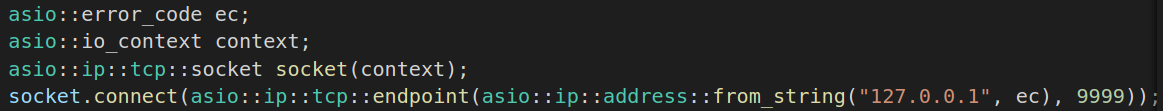
\includegraphics[width=\textwidth]{clientep.png}
    \caption{Client Socketverbindung}
\end{figure}
\end{center}

Die Wahl des Ports beruht auf einem Leitfaden zur Auswahl von Ports bei Networking-Programmierung, der Port 9999 wurde auf Seiten von TCP und UDP nicht besonders spezifiziert oder besetzt. Nachzulesen unter:\\ \textbf{https://en.wikipedia.org/wiki/List\_of\_TCP\_and\_UDP\_port\_numbers}
\\
\newline
Danach wird geloggt, dass der Client sich mit dem Server verbunden hat und die Datenübertragung beginnt. Es werden zuerst die Größe der Fenster geschickt und die Anzahl aller Datenframes geschickt. Der Client speichert die schon vorhin beschriebene MAX\_SUM aller Daten zwischen und beginnt nun mit der Übertragung der eigentlichen ASCII-Zeichen jeweils in Anzahl der Fenstergröße auf einmal.

Der Client überprüft, ob der Server die richtigen AKN sendet und lässt so das Fenster weiter gleiten. Falls ein falscher AKN kommen, wird ein Fehler geloggt, und das Programm fährt fort. Am Ende empfängt der Client die MAX\_SUM des Server, wenn diese mit der vorhin zwischengespeicherten des Clients übereinstimmt, kommt eine Nachricht, dass die Übertragung ohne Probleme vollzogen werden konnte. Falls nicht, wird dies auch entsprechend geloggt und ausgegeben. Der gesamte Vorgang wird auf Client und Serverseite in zwei seperate Logdateien geschrieben. Der Pfad für die des Clients steht in der settings.json Datei im \textbf{/build} - Verzeichnis. Die des Server ist fix im Code angegeben, und zwar immer im aktuellen Verzeichnis, wo sich die ausführbare Datei des Servers beim starten befindet.

\subsection{Umsetzung Server}

Wenn der Server gestartet wird, wird zuerst ein Endpoint erstellt und ein \textbf{asio::acceptor} listened auf neue Verbindungen. Danach wird der Logger erstellt wie in Abb. 9 zu sehen ist.

\begin{center}
\begin{figure}[h]
    \centering
    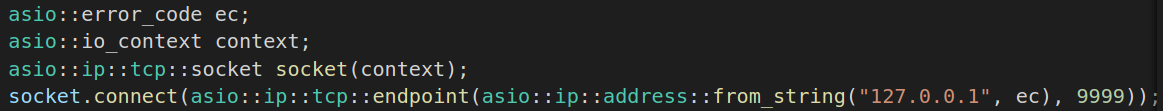
\includegraphics[width=\textwidth]{clientep.png}
    \caption{Server Listen}
\end{figure}
\end{center}

In einer Endlos-Schleife, erzeugt der Server dann mit ankommenden Verbindungen einen Socket und akzeptiert sie. Falls dies ohne Fehler funktioniert startet er für jeden Socket einen Thread, welcher die Funktion \textbf{process()} ausführen muss.

\begin{lstlisting}
void process(asio::ip::tcp::socket socket,
std::shared_ptr<spdlog::logger> logger)
\end{lstlisting}

Diese Funktion erwartet eine ein Socket-Objekt und ein ein \textbf{shared\_pointer} vom Typ \textbf{spdlog::logger}. Dieser Ablauf ist in Abb. 10 zu sehen.

\begin{center}
\begin{figure}[h]
    \centering
    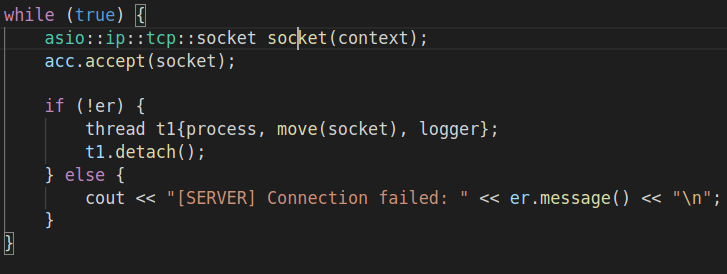
\includegraphics[width=\textwidth]{servercon.png}
    \caption{Server Eingehende Verbindung}
\end{figure}
\end{center}

In der Funktion \textbf{process()} wird zuerst die die Sliding Window Fenstergröße empfangen, dann die Anzahl aller zu Erwartenden Daten. Später, vor der Verarbeitung der eigentlichen ASCII Werte wird noch eine Uhrzeit gespeichert und bei jedem Schleifendurchlauf wird diese mit der aktuellen Zeit am Server verglichen, der gesamte Prozess darf aus Sicherheitsgründen nicht mehr als sechs Sekunden dauern. Falls diese Zeit überschritten wird, wird beim nächsten Schleifendurchlauf das Socket geschlossen, und es können auf diesem keine Daten mehr gesendet und empfangen werden.\\
Der Server loggt alle Ereignisse und gibt den Ablauf auch in der Konsole aus. Jeden AKN und die aktuelle Checksumme des Algorithmus. Am Ende wird mit der \textbf{max\_sum} noch die größte Summe berechnet und übertragen. Danach beendet der Server den Socket nach einer 90 Millisekunden langen Wartezeit. Dies ist aufgrund von Performance und des speziellen Programmablaufes künstlich erzeugt worden.

\break

\section{Verwendete Externe Klassen}
\begin{itemize}
	\item \underline{rang-library:} für die farbige Ausgabe der Tabelle
	\item \underline{CLI11-library:} für die Verarbeitung von Eingabe und Options- und Funktionsargumenten
	\item \underline{spdlog-library:} für das Logging
	\item \underline{tabulate-library:} für die Formatierung der Ausgabe als Tabelle
	\item \underline{asio-library:} für das networking in C++
	\item \underline{chrono-library:} für Zeitmessungen
	\item \underline{json-library:} JSON for modern C++ für die Änderung des Logpfades und Speicherung dessen
\end{itemize}


\section{Quellen}

\begin{itemize}
	\item \underline{https://tools.ietf.org/html/rfc1180}
	\item \underline{https://justtechreview.com/sliding-window-protocol-program-in-c-and-c/}
	\item \underline{https://tools.ietf.org/html/rfc1180\#section-7}
	\item \underline{https://www.tutorialspoint.com/sliding-window-protocol}
	\item \underline{https://www.geeksforgeeks.org/window-sliding-technique/}
	\item \underline{https://www.cplusplus.com/reference/vector/vector/max\_size/}
	\item \underline{https://stackoverflow.com/questions/32316346/limit-on-vectors-in-c}
	\item \underline{Folie distsys1.pdf aus dem NVS Unterricht und Folie 26-, 27- und 28\_tcpip\_programming.pdf}
\end{itemize}

\textbf{Alle benutzen Bilder sind frei für akademische Zwecke zu benutzen oder das Urheberrecht liegt beim Verfasser (Maurice Putz)}

\end{document}